\documentclass[11pt]{article}
    \usepackage{caption}
    \usepackage{graphicx}
    \usepackage{mathtools}
    \usepackage{bookmark}
    \graphicspath{ {img/} }
    \setlength{\parindent}{0pt}
    \DeclareCaptionType{equ}[][]
    \usepackage[svgnames]{xcolor}
    \graphicspath{ {./img/} }

    
    \newcommand*{\plogo}{\fbox{$\mathcal{BM}$}}
    
    \usepackage{PTSerif}
    
    \begin{document} 
        
    \begin{titlepage}
    
        \raggedleft
        
        \vspace*{\baselineskip}
        
        {\Large Bryan Melanson}
        
        \vspace*{0.167\textheight}
        
        \textbf{\LARGE How to Not Fail}\\[\baselineskip]
        
        {\textcolor{Red}{\Huge Computer Architecture}}\\[\baselineskip]
        
        {\Large \textit{While never going to class}}
        
        \vfill
        
        {\large Computer Engineering 2020 ~~\plogo}
        
        \vspace*{3\baselineskip}
    
    \end{titlepage}

    \pagebreak
    
%%%%%%%%%%%%%%%%%%%%%%%%%%%%%%%%%%%%%%%%%%%%%%%%%
    \pdfbookmark[section]{\contentsname}{toc}
    
    \tableofcontents

%%%%%%%%%%%%%%%%%%%%%%%%%%%%%%%%%%%%%%%%%%%%%%%%%

\section{Introduction}

\subsection{RISC}

\textbf{RISC} (Reduced Instruction Set Computer) is an architecture which allowed for the exploitation of instruction level parallelism and the use of caches. This increased performance couldn't be matched by other architectures, and Intel 80x86 was forced to translate its instructions into RISC-like form internally to adopt RISC innovations. In low-end applications, this has lead to RISC architecture like ARM becoming dominant.

\subsection{Dennard Scaling}

Power density was a constant for a given area of silicon, even as the number of transistors increased, due to their smalll dimension. This held up until a certain level in 2004, when the current and voltage levels could no longer ensure the dependability of integrated circuits.

\subsection{Multiple Processors}

The end of Dennard Scaling meant that improve performance more processors would be implemented, since single core chips would be inefficient with the increasing number of transistors. This meant that designs would no longer rely on \textbf{Instruction Level Parallelism}.

\subsection{Classes of Parallelism}

\begin{itemize}
    \item \textbf{Data Level Parallelism} - data items operated on at the same time
    \item \textbf{Task Level Parallelism} - tasks performed independently in parallel
\end{itemize}

\subsection{Application Parallelism}

\begin{itemize}
    \item \textbf{Instruction Level Parallelism} - exploits data-level using pipelining and speculative execution
    \item \textbf{Vector Archictectures} - exploits data-level parallelism using single instructions on a collection of data in parallel
    \item \textbf{Thread Level Parallelism} - data or task-level parallelism allowing for interaction between parallel threads
    \item \textbf{Request Level Parallelism} - parallelism between decoupled tasks
\end{itemize}

\subsection{Flynn's Taxonomy}

\begin{itemize}
    \item \textbf{Single Instruction Stream, Single Data Stream} - a single processor operates on sequential computation but can exploit ILP
    \item \textbf{Single Instruction Stream, Single Data Stream} - the same instruction executed by multiple processors, uses data level parallelism
    \item \textbf{Multiple Instruction Streams, Single Data Stream} - no implementation to date
    \item \textbf{Multiple Instruction Streams, Multiple Data Stream} - processesors have their own instructions and own data operated on, using task level parallelism. Used in warehouse level computing, exploiting request level parallelism where many independent tasks can proceed in parallel
\end{itemize}

\subsection{Warehouse Scale Computers}

Warehouse Scale Computers \textbf{WSC}s are collections of servers or \textbf{clusters} which Software as a Service (SaaS) uses as a single larger computer, capable of considerable processing power. Price-performance and power are critical.

\subsection{Instruction Set Architecture}

The old view of computer architecture focused on \textbf{Instruction Set Architecture} (ISA) design involves decisions regarding registers, memory addressing, addressing modes, instruction operands, available operations, control instructions and instruction encoding.\\

Computer architecture now involves specific requirements of the target machine, designs meant to maximize performance within constraints, ISA, microarchitecture, and requires consideration of how compilers work.

\subsection{RISC-V Instruction Formats}

\begin{center}
    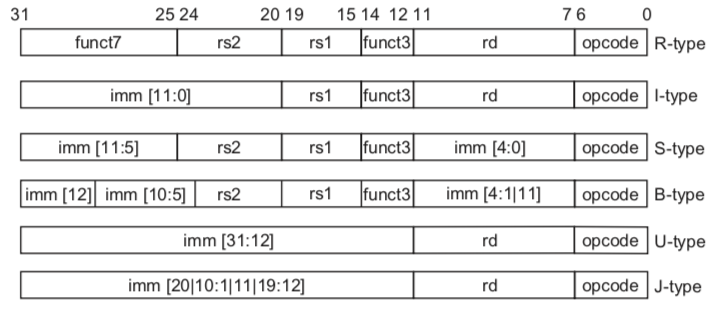
\includegraphics[scale=0.5]{riscv_formats}
\end{center}

The above represents the format of different binary instruction types. The values $rs2$, $rs1$, $rd$, etc. represent the binary values which will specify which registers are targetted by the instruction. Values $funct$ and $opcode$ will describe which operation to execute, and $imm$ fields will hold immediate values as arguments. 

\subsection{Latency and Bandwidth}

Latency and Bandwidth are valuable performance metrics. Latency is the responsiveness with which commands can be executed; the time between start and completion of an event. Bandwidth is the total work done in a given time. Bandwidth and capacity have been more valued in the past, and in general show a greater growth rate - the growth of bandwidth is generally the square of the improvement in latency.

\subsection{Dynamic State Energy and Power}

\textbf{Dynamic Energy} is the switching of transistors to conserve energy. This value is therefore proportional to the product of the capactive load and the square of the voltage:

\begin{center}
    Energy$_{dynamic}$ $\propto$ Capacitive Load $\cdot$ Voltage$^2$
\end{center}

This represents the energy of a pulse from 0 $\rightarrow$ 1 $\rightarrow$ 0, or vice verse, so the value of each single transition is:

\begin{center}
    Energy$_{dynamic}$ $\propto$ $\frac{1}{2}$ Capacitive Load $\cdot$ Voltage$^2$
\end{center}

And the Dynamic Power is:

\begin{center}
    Power$_{dynamic}$ $\propto$ $\frac{1}{2}$ Capacitive Load $\cdot$ Voltage$^2$ $\cdot$ Frequency Switched
\end{center}

\subsection{Die Yield}

\begin{center}
    \begin{equation}
    \text{Die Yield} = (1 + (\frac{\text{Defects/Area} \cdot \text{Area of Die}}{N}))^{-N}
    \end{equation}
\end{center}

\textbf{Die Yield} is a value which defines how likely it is that a die will be non-defective during the fabrication process. This value is a probability $< 1$, and the probability that a die will be defective is $1 - $Die Yield. \\
When converting between units of area (mm$^2$, cm$^2$), be sure to repeat conversion between units twice.

\begin{center}
    1 mm$^2$ = $\frac{1}{10 \text{cm}} \cdot \frac{1}{10 \text{cm}} = \frac{1}{100}$ cm$^2$
\end{center}

\subsection{Wafer Yield}

\textbf{Wafer Yield} is a value which describes how many dies (chips) can be created from a single wafer. This calculation is done using the size of a chip, and the diameter of each wafer. It takes into effect the square or rectangle shape of a chip and losses due to rounded sides of a wafer.

\begin{center}
\begin{equation} \text{Dies per wafer} = 
    \frac{\pi \cdot (\text{Wafer Diameter}/2)^2}{\text{Die area}} - \frac{\pi \cdot \text{Wafer diameter}}{\sqrt{2 \cdot \text{Die area}}}    
\end{equation}
\end{center}

These values can be used to calculate the cost of each die:

\begin{center}
    Cost of die = $\frac{\text{Cost of wafer}}{\text{Dies per wafer}\cdot\text{Die yield}}$
\end{center}

\subsection{Dependability}

\begin{itemize}
    \item \textbf{Mean Time to Failure (MTTF)} - How long is continuous service delivered, the reciprocal is the rate of failure. One failure for every length of time.
    \item \textbf{Mean Time to Repair (MTTR)} - How long is service interruption
    \item\textbf{Availability = MTTF / (MTTF + MTTR)} - Service is continuous for $x$ amount of time for every $y$ length, MTTF + MTTR.
\end{itemize}

\subsection{Performance}

Performance metrics can differ between computers and their purposes - WSCs will want to increase bandwidth, and mobile devices will want to increase the speed with which commands are executed. 

\begin{center}
    $\frac{\text{Execution time}_Y}{\text{Execution time}_X}$ = $n$ = $\frac{\text{Performance}_X}{\text{Performance}_Y}$
\end{center}

\subsubsection{Execution Time}

\textbf{Amdahl's Law} states that the performance improvement to be gained from using some fasted mode of execution is limited by the fraction of time the faster mode can be used.

\begin{center}
    Speedup = $\frac{\text{Performance for entire task using enhancement when possible}}{\text{Performance for entire task without using the enhancement}}$
\end{center}

The speedup depends on two factors:

\begin{enumerate}
    \item The fraction of computation time in the original computer that can be converted to take advantage of the enhancement - Fraction$_{\text{enhanced}}$
    \item How much faster the task would run if the entire program were enhanced - Speedup$_{\text{enhanced}}$
\end{enumerate}

\begin{center}
    {Exec Time}$_\text{new}$ = {Exec Time}$_\text{old}$ $\cdot$ ((1 - Fraction$_\text{enhanced}$) + $\frac{\text{Fraction}_\text{enhanced}}{\text{Speedup}_\text{enhanced}}$)
\end{center}

The above equation cancels in several points to be equal to 

\begin{center}
    Execution Time$_\text{old}$ $\cdot$ Old Code + Execution Time$_\text{new}$ $\cdot$ New Code
\end{center}

\begin{center}
    {Speedup}$_\text{new}$ = $\frac{\text{Execution Time}_\text{old}}{\text{Execution Time}_\text{new}}$
\end{center}

\begin{center}
    {Speedup}$_\text{new}$ = $\frac{1}{(1-\text{Fraction}_\text{enhanced}) + \frac{\text{Fraction}_\text{enhanced}}{\text{Speedup}_\text{enhanced}}}$
\end{center}

\subsubsection{Processor Performance Equation}

\begin{center}
    CPU Time = CPU Clock Cycles for a Program $\cdot$ Clock Cycle Time
\end{center}

Clock cycles can also be defined as $\textbf{Instruction Count} \cdot \textbf{Clock Cycle Time}$

\begin{center}
    CPU Time = Instruction Count $\cdot$ Cycles per Instruction $\cdot$ Clock Cycle Time
\end{center}

\section{Instruction Set Architecture}

Memory is \textbf{byte addressable} in major architecture types - all bytes have a unique address, which allows for units as small as an ASCII character to be accessed without using larger accesses and masking. \\

ISA's should allow access commands for loading and writing byte, half words, and words so that units such as integers, and longs can be accessed and modified with ease. \\

\begin{tabular}{ l r}
    Byte & 8 bits \\ 
    Half Word & 16 bits \\
    Word & 32 bits \\
    Double Word & 64 bits
\end{tabular}
\\ \\
\textbf{Little Endian} orders bytes in a larger object such that the byte ending 000 will be found at the LSB position \\ \\
    \begin{tabular}{ c c c c c c c c }
        7 & 6 & 5 & 4 & 3 & 2 & 1 & 0
    \end{tabular} \\ \\ 
\textbf{Big Endian} orders bytes so that the byte ending 000 will be located in the MSB position \\ \\
    \begin{tabular}{ c c c c c c c c }
        0 & 1 & 2 & 3 & 4 & 5 & 6 & 7
    \end{tabular} \\ \\ 
    
\end{document}
